\documentclass[11pt,a4paper]{article}
\usepackage[margin=20mm]{geometry}
\usepackage{amsmath,graphicx,caption}
\setlength{\parindent}{0pt}
\setlength{\parskip}{5pt}
\begin{document}
\begin{center}
{\Large\bfseries Experiment 8: Buck Converter}\\[6pt]
Lataksh Sariya \quad EE24BT018
\end{center}
\section*{Aim}
To design and test a buck converter using the TL494 PWM module.
\section*{Specifications}
Input: 15--25 V (20 V nominal), output: 10 V, switching frequency: 25 kHz, rated output power: 100 W. The current and voltage ripples are taken as 0.2 A and 0.1 V peak-to-peak.
\section*{Theory and calculations}
A buck converter gives a lower DC output voltage by controlling the switch duty ratio. The inductor and capacitor smooth the switched waveform. For ideal operation,
\[
V_o=DV_{in},\qquad D=\frac{10}{20}=0.5=50\%.
\]
The switching period is $T=1/(25\times10^3)=40\,\mu\mathrm{s}$, so the ON and OFF times are both $20\,\mu\mathrm{s}$ at the nominal input.

The rated output current and load resistance are
\[
I_o=\frac{P_o}{V_o}=\frac{100}{10}=10\,\mathrm{A},
\qquad R=\frac{V_o^2}{P_o}=\frac{10^2}{100}=1\,\Omega.
\]
The required inductance at 20 V is
\[
L=\frac{(V_{in}-V_o)D}{f_s\Delta I_L}
=\frac{(20-10)\times0.5}{25000\times0.2}
=\boxed{1\,\mathrm{mH}}.
\]
Neglecting capacitor ESR, the minimum output capacitance is
\[
C=\frac{\Delta I_L}{8f_s\Delta V_o}
=\frac{0.2}{8\times25000\times0.1}
=\boxed{10\,\mu\mathrm{F}}.
\]
For the practical inductor, $L=0.95$ mH, the expected current ripple at 20 V is
\[
\Delta I_L=\frac{(20-10)\times0.5}{25000\times0.95\times10^{-3}}
\approx\boxed{0.211\,\mathrm{A}}.
\]
These calculations are for the nominal input. To meet the 0.2 A current-ripple limit throughout 15--25 V, the required inductance is at least 1.2 mH.
\section*{Procedure and observations}
The converter was operated using a TL494 module, an IRF540N MOSFET, a fast recovery diode and the 0.95 mH inductor. The waveforms were recorded on the oscilloscope. The probable gate waveform shows 26.04 kHz and 53.71\% duty. The likely output-voltage trace has a mean of 10.12 V. Switching spikes are visible in the pulse waveform. The probe points are not labelled in the photographs, so these signal identifications are inferred.
\section*{Result}
The recorded output is consistent with the 10 V target. The practical inductor gives a calculated ripple close to the specified 0.2 A at nominal input. Current ripple and 100 W output operation were not verified from the available photographs.
\newpage
\section*{Recorded waveforms}
\begin{minipage}[t]{0.48\linewidth}
\centering
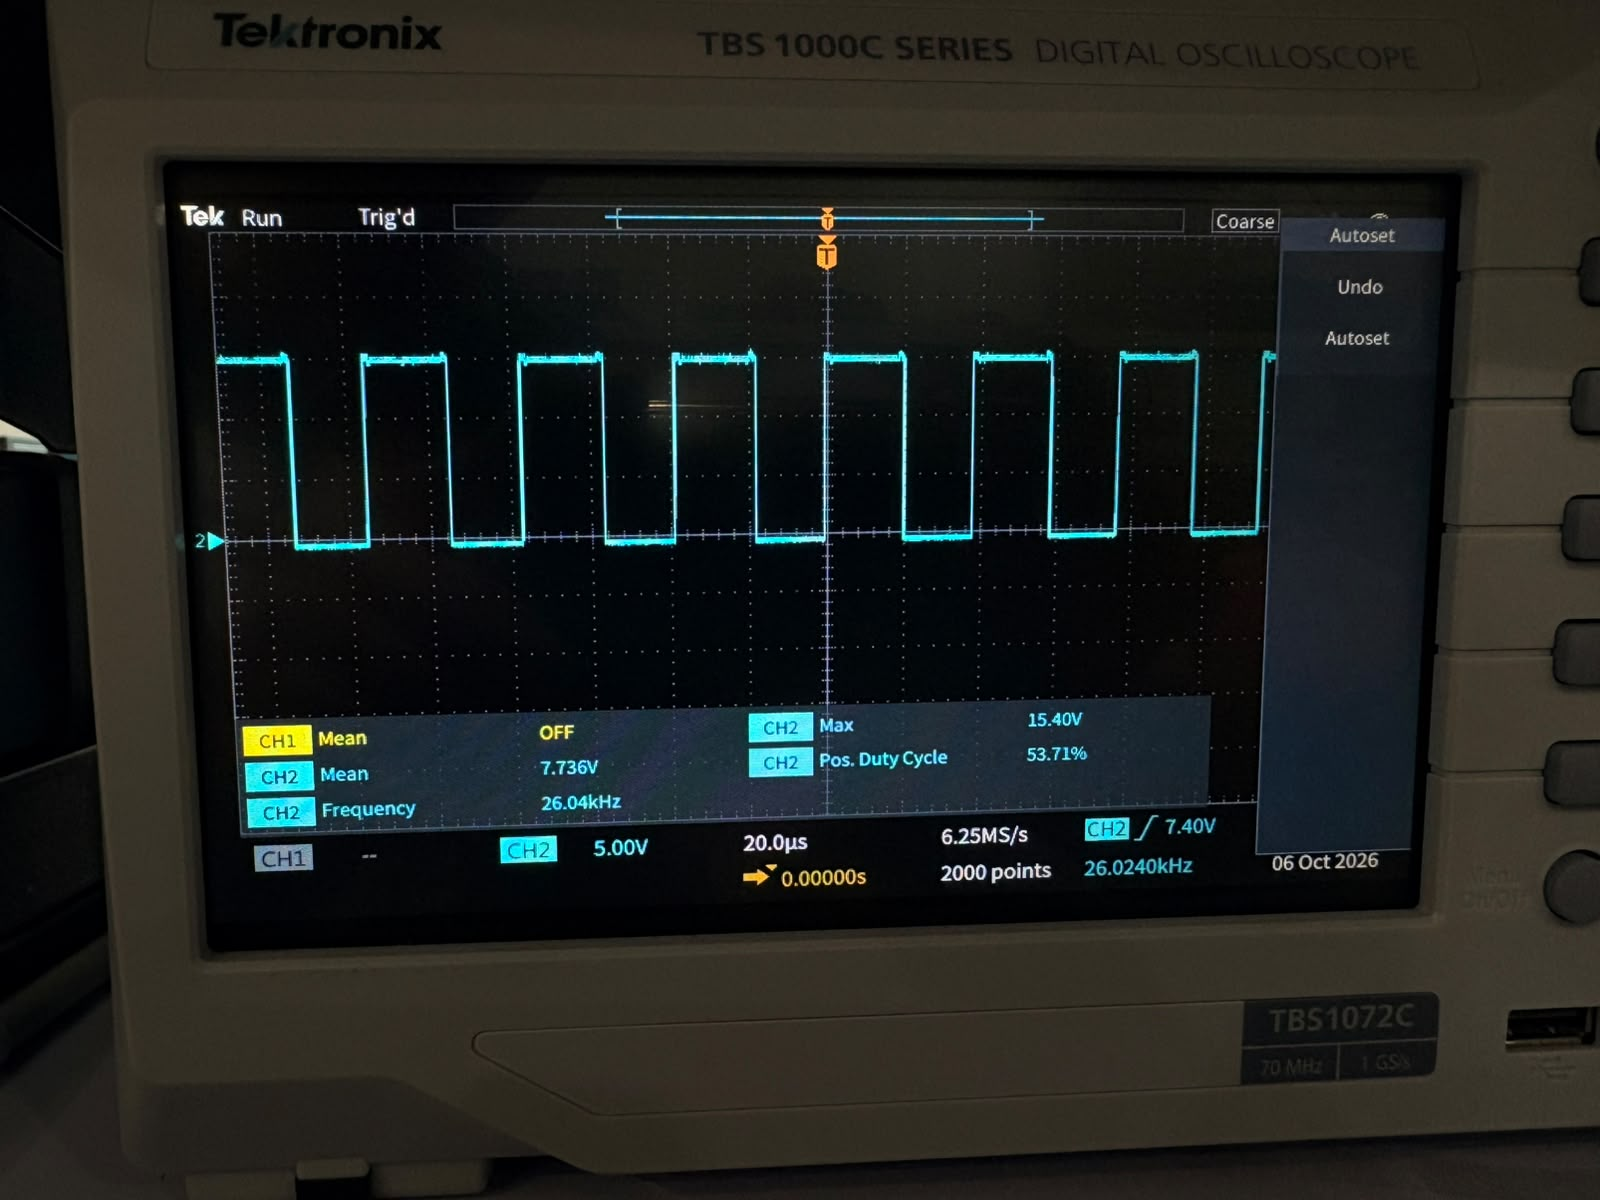
\includegraphics[width=\linewidth]{images/photo10.jpg}
\captionof{figure}{Probable gate pulses: 26.04 kHz, 53.71\% duty.}
\end{minipage}\hfill
\begin{minipage}[t]{0.48\linewidth}
\centering
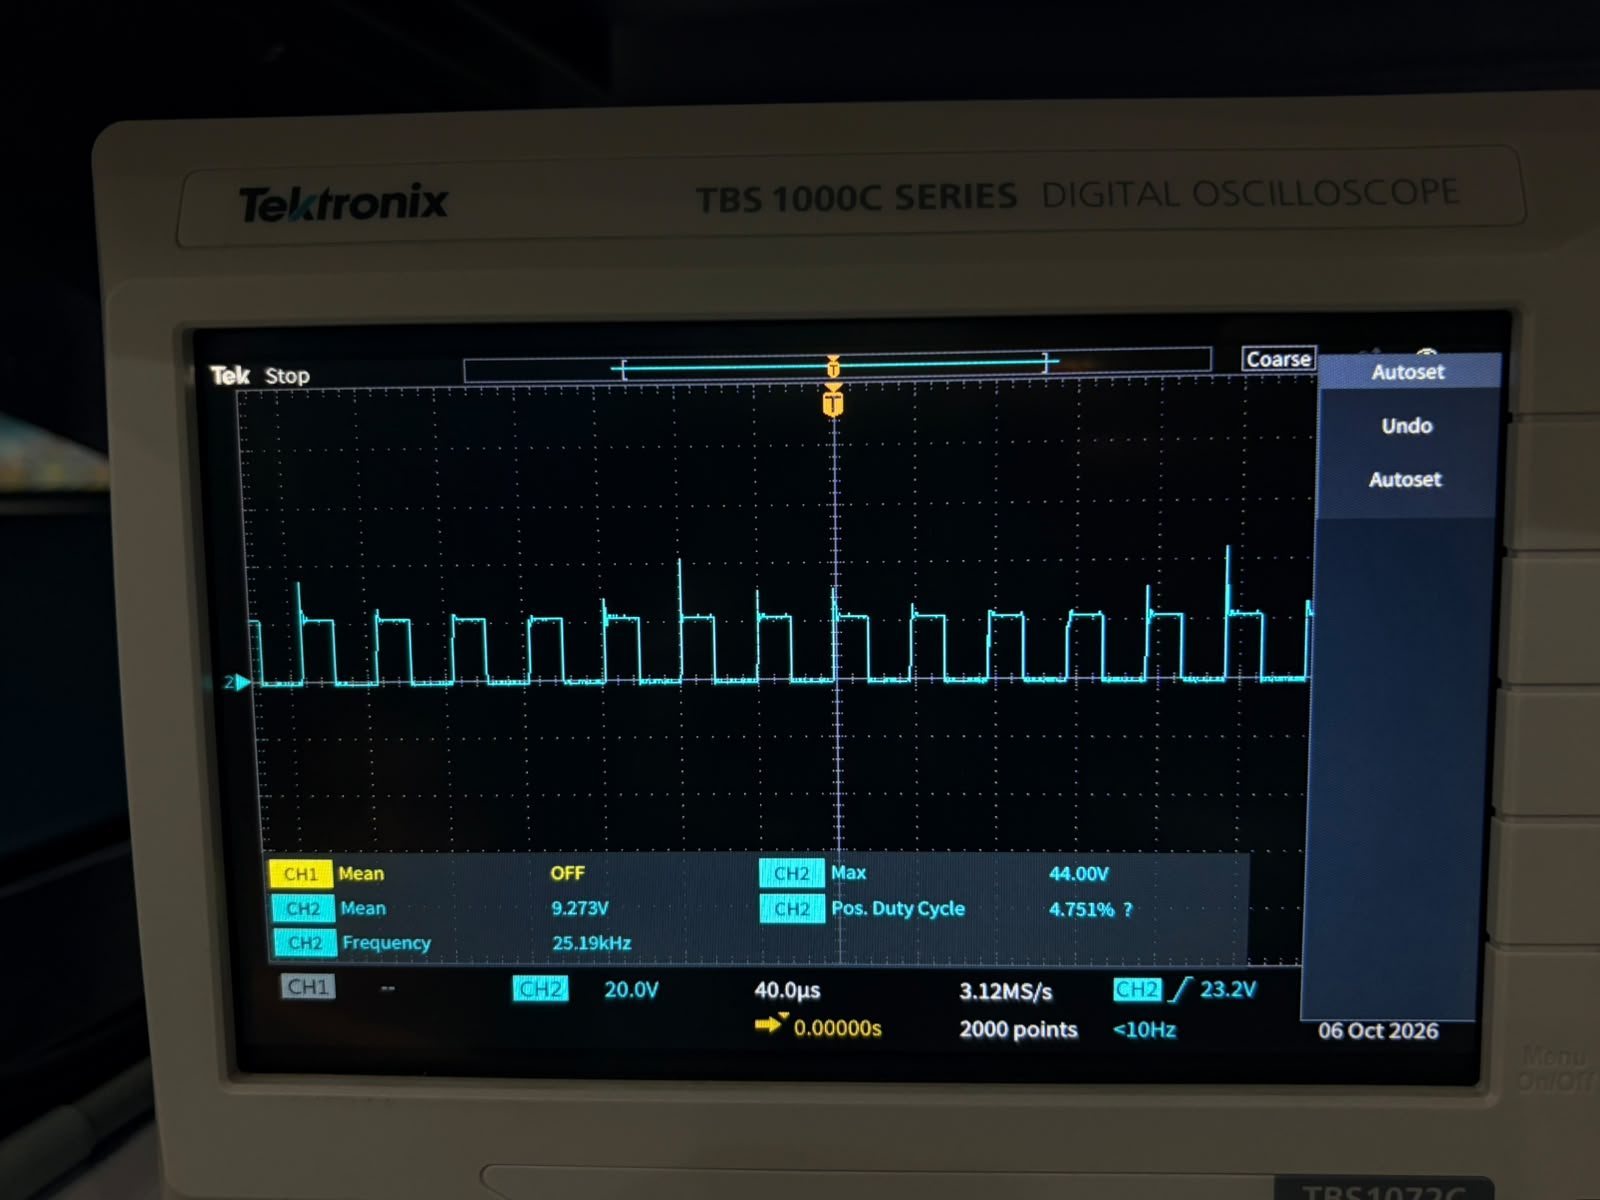
\includegraphics[width=\linewidth]{images/photo08.jpg}
\captionof{figure}{Switching-voltage waveform with spikes. Exact probe point is unknown.}
\end{minipage}
\vspace{12mm}
\begin{center}
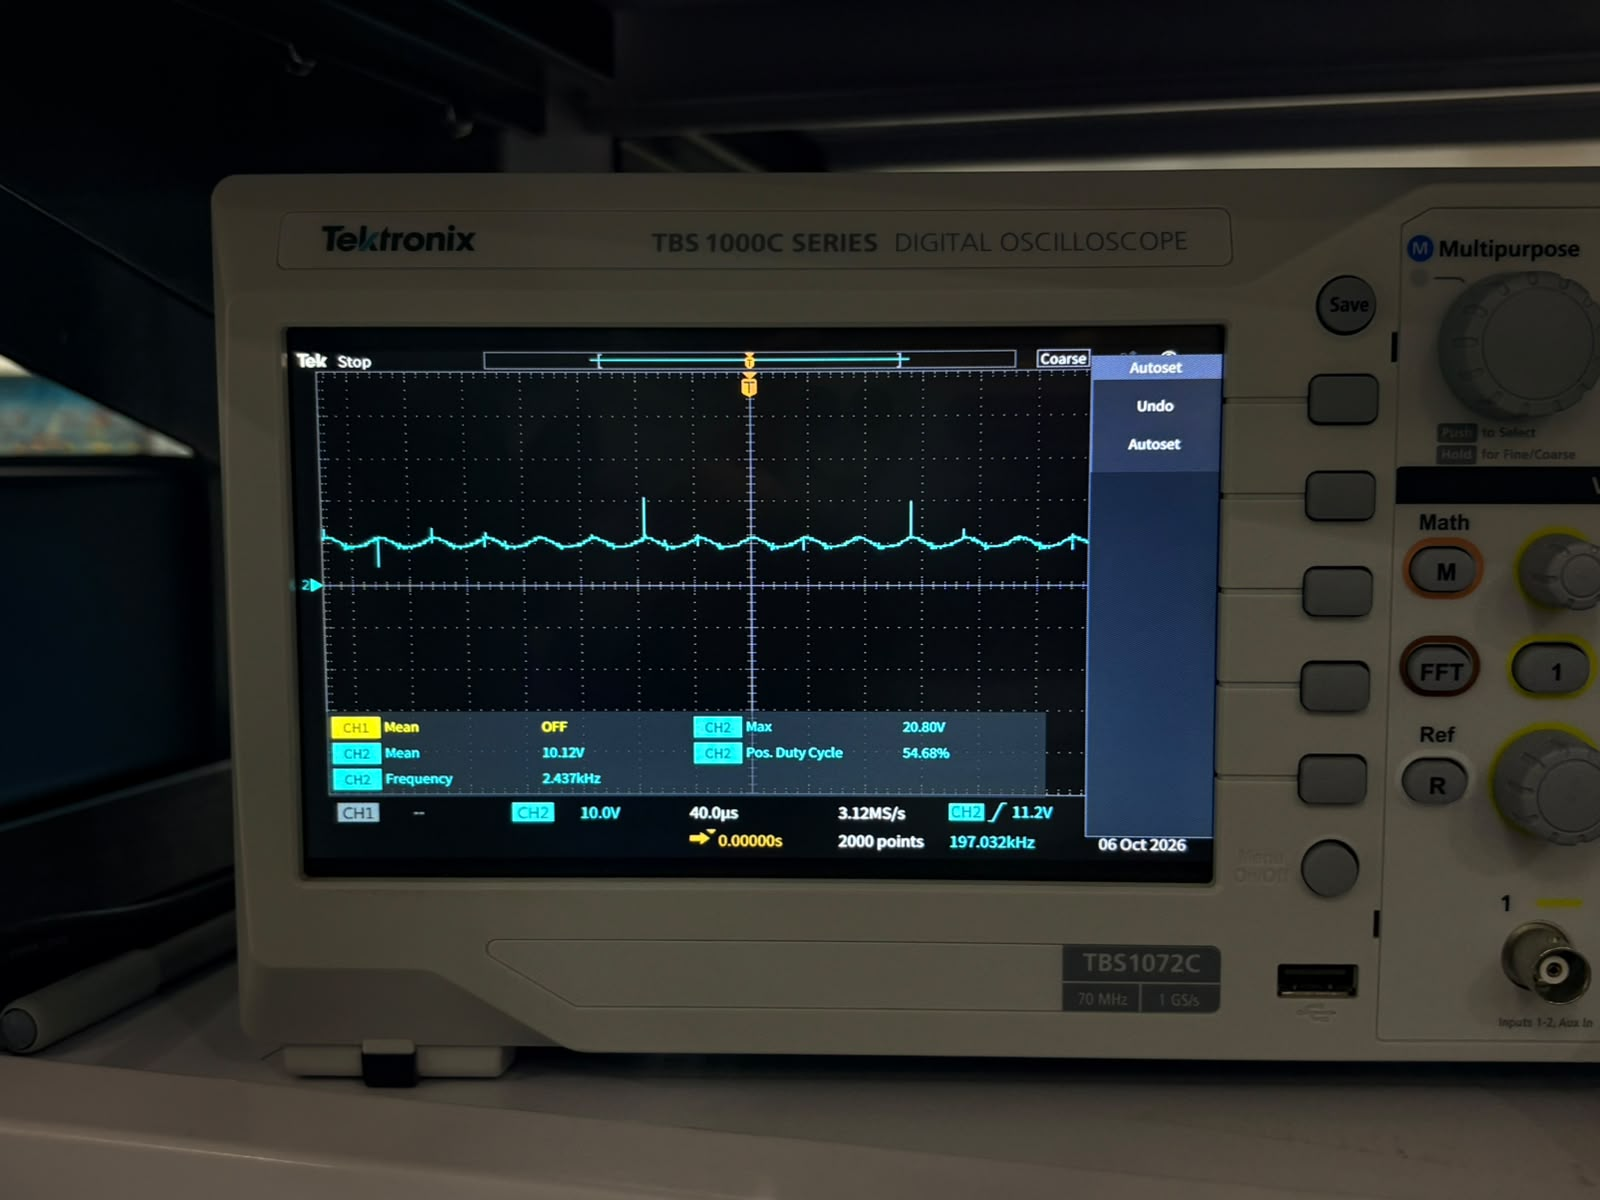
\includegraphics[width=0.88\linewidth]{images/photo06.jpg}
\captionof{figure}{Probable output voltage. The displayed mean is 10.12 V.}
\end{center}
The photographs show PWM switching and an approximately DC output. Some automatic readings on the noisy traces are unreliable; the output ripple cannot be checked accurately at the displayed scale.
\vfill
{\small Reference: DPC 2026 Experiment 8 laboratory sheet.}
\end{document}
